\section{Results}
\label{sec:results}

Cosmological constraints

\begin{figure}
	\begin{center}
		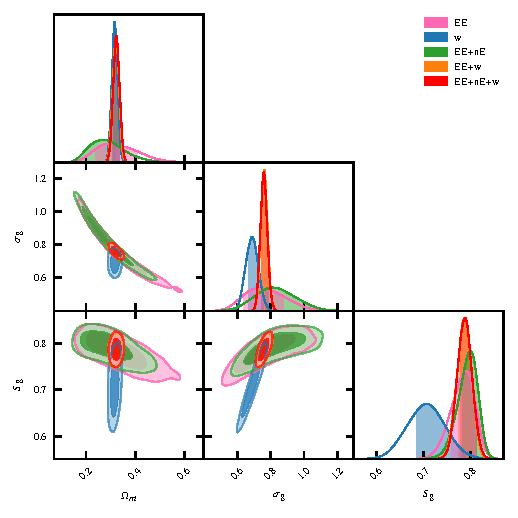
\includegraphics[width=\columnwidth]{Parameter_Plots/omegam_sigma8_s8_blind_A}
		\caption{Constraints on flat $\Lambda$CDM blind A}
		\label{fig:cosmology-params}
	\end{center}
\end{figure}

\begin{figure}
	\begin{center}
		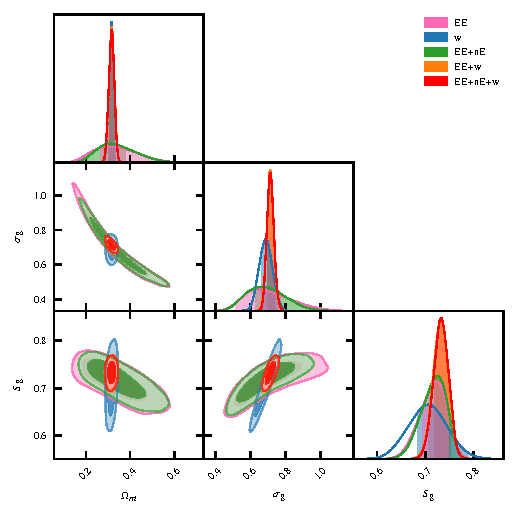
\includegraphics[width=\columnwidth]{Parameter_Plots/omegam_sigma8_s8_blind_B}
		\caption{Constraints on flat $\Lambda$CDM blind B}
		\label{fig:cosmology-params}
	\end{center}
\end{figure}

\begin{figure}
	\begin{center}
		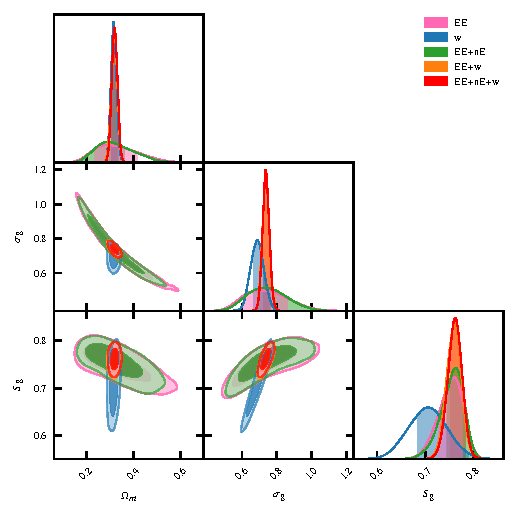
\includegraphics[width=\columnwidth]{Parameter_Plots/omegam_sigma8_s8_blind_C}
		\caption{Constraints on flat $\Lambda$CDM blind C}
		\label{fig:cosmology-params}
	\end{center}
\end{figure}


\begin{figure}
	\begin{center}
		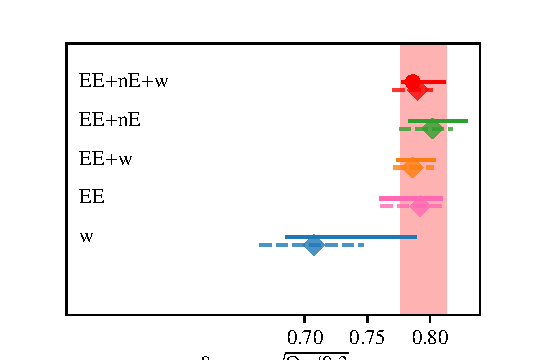
\includegraphics[width=\columnwidth]{Parameter_Plots/S8_comparison_blindA}
		\caption{Constraints on $S_{8}$ blind A}
		\label{fig:cosmology-params}
	\end{center}
\end{figure}

\begin{figure}
	\begin{center}
		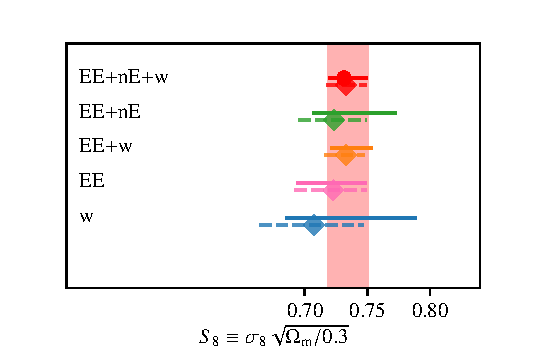
\includegraphics[width=\columnwidth]{Parameter_Plots/S8_comparison_blindB}
		\caption{Constraints on $S_{8}$ blind B}
		\label{fig:cosmology-params}
	\end{center}
\end{figure}

\begin{figure}
	\begin{center}
		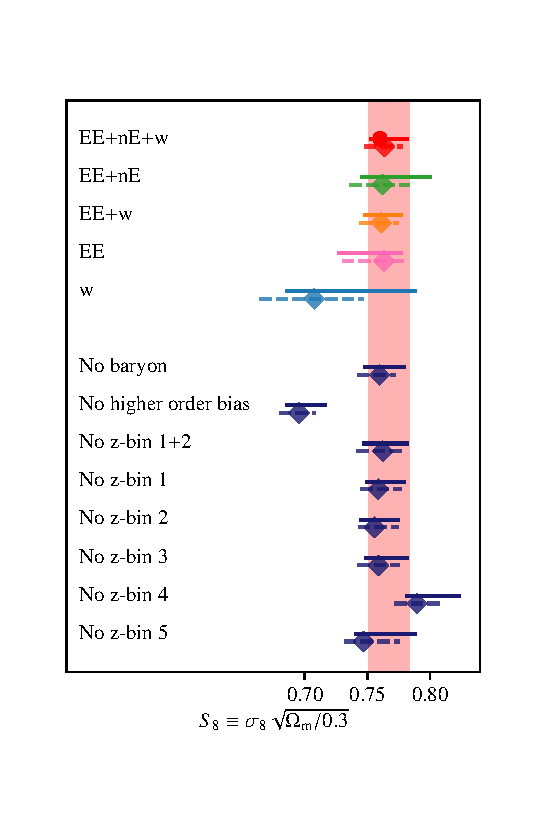
\includegraphics[width=\columnwidth]{Parameter_Plots/S8_comparison_blindC}
		\caption{Constraints on $S_{8}$ blind C}
		\label{fig:cosmology-params}
	\end{center}
\end{figure}

\begin{figure*}
	\begin{center}
		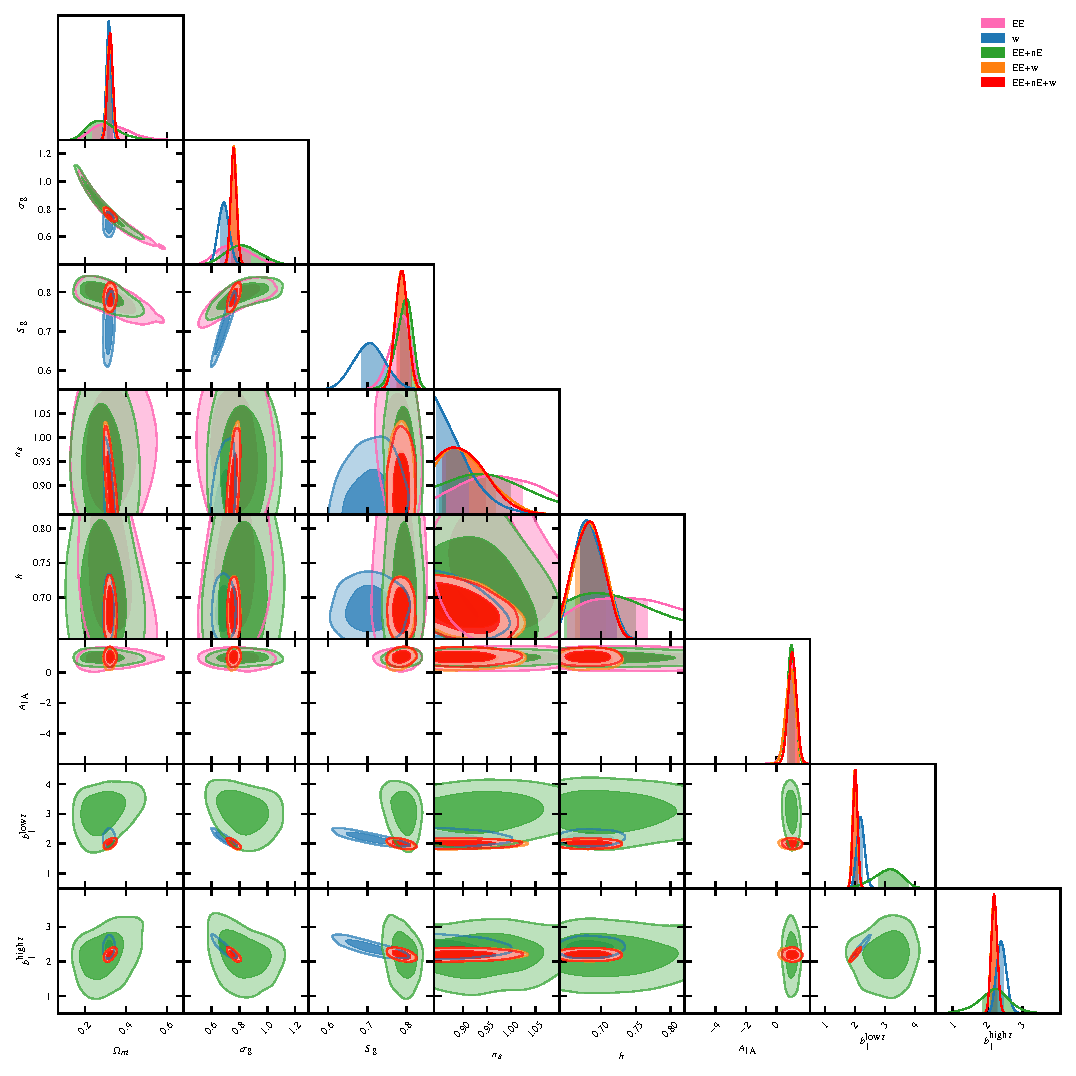
\includegraphics[width=\textwidth]{Parameter_Plots/omegam_sigma8_s8_ns_h_a_ia_b1l_b1h_blind_A}
		\caption{Constraints blind A}
		\label{fig:cosmology-params}
	\end{center}
\end{figure*}

\begin{figure*}
	\begin{center}
		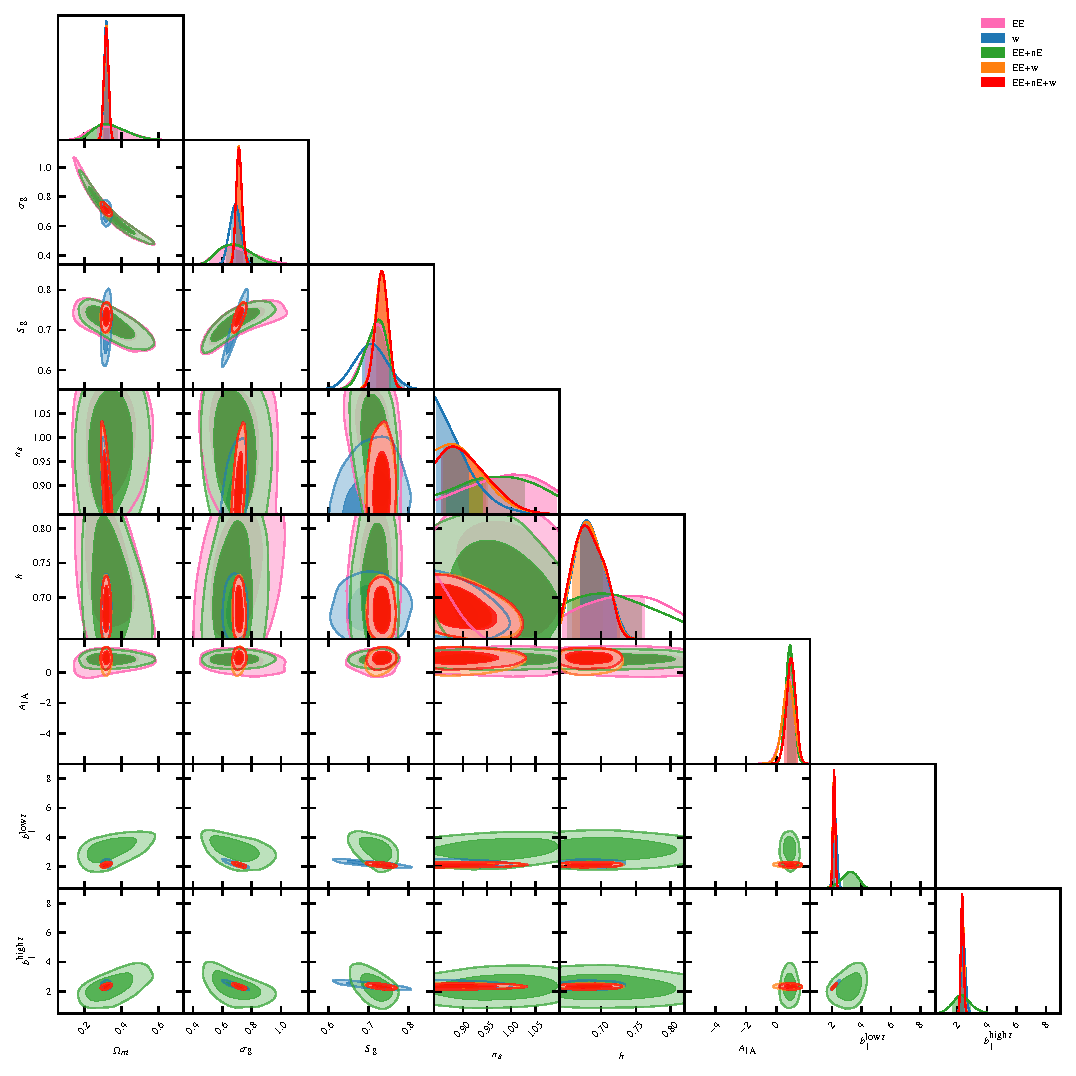
\includegraphics[width=\textwidth]{Parameter_Plots/omegam_sigma8_s8_ns_h_a_ia_b1l_b1h_blind_B}
		\caption{Constraints blind B}
		\label{fig:cosmology-params}
	\end{center}
\end{figure*}

\begin{figure*}
	\begin{center}
		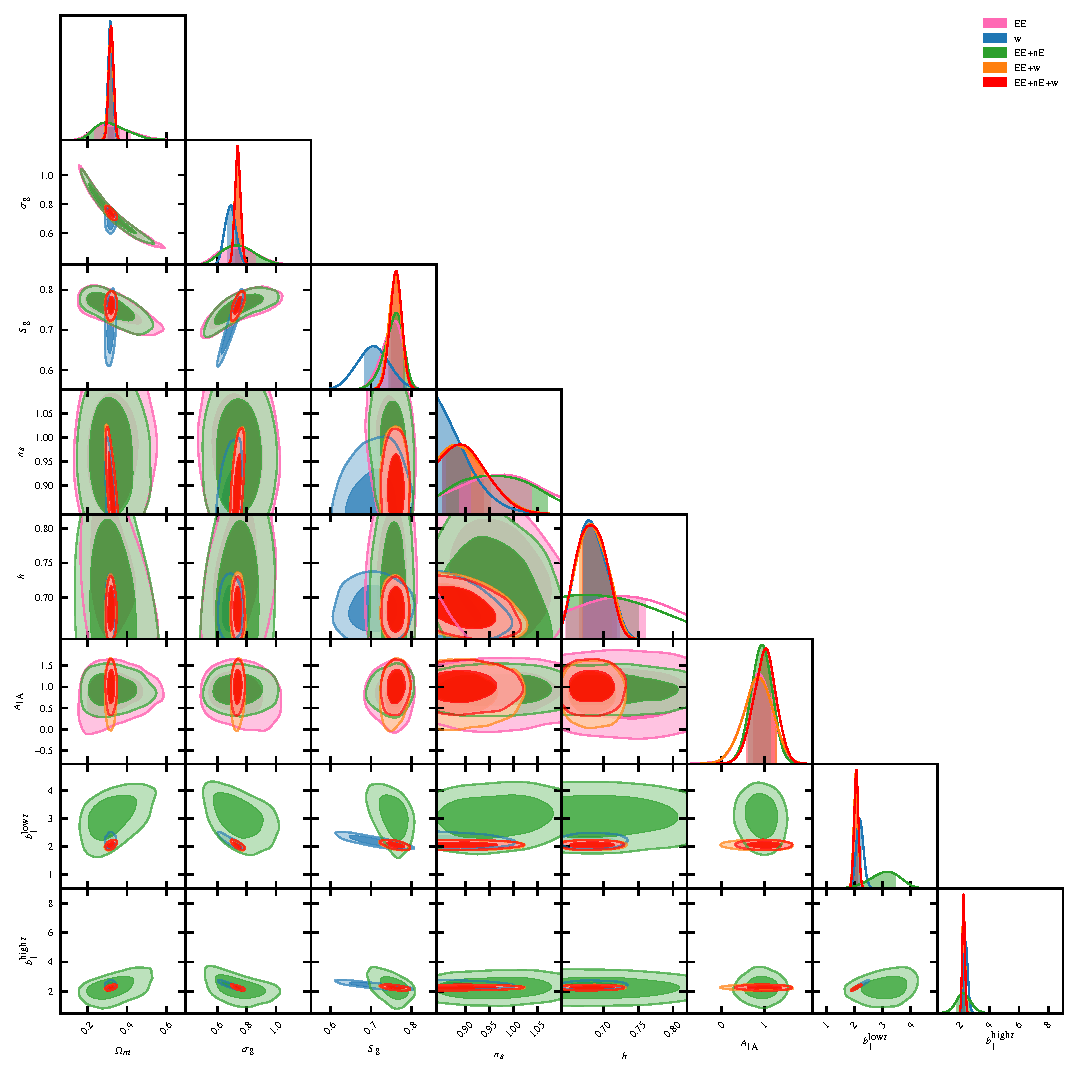
\includegraphics[width=\textwidth]{Parameter_Plots/omegam_sigma8_s8_ns_h_a_ia_b1l_b1h_blind_C}
		\caption{Constraints blind C}
		\label{fig:cosmology-params}
	\end{center}
\end{figure*}

\begin{table}
	\begin{center}
		\caption{Goodness of fit for blind A}
		\label{tab:goodness-of-fit}
\begin{tabular}{lrcl}
    \toprule
    Probe             & $\chi^2$       & ndof       & PTE   \\
    \midrule
	EE               & $< 156.1$ & $120-4.5$ & 0.000 \\
	w                & $< 196.1$ & $168-42.0$ & 0.000 \\
	EE+nE            & $< 217.2$ & $ 42-42.0$ & 0.000 \\
	EE+w             & $< 365.4$ & $ 42-42.0$ & 0.000 \\
	EE+nE+w          & $409.8$ & $ 42-42.0$ & 0.000 \\
    \bottomrule
\end{tabular}
	\end{center}
\end{table}

\begin{table}
	\begin{center}
		\caption{Goodness of fit for blind B}
		\label{tab:goodness-of-fit}
\begin{tabular}{lrcl}
    \toprule
    Probe             & $\chi^2$       & ndof       & PTE   \\
    \midrule
	EE               & $< 148.1$ & $120-4.5$ & 0.000 \\
	w                & $< 196.1$ & $168-42.0$ & 0.000 \\
	EE+nE            & $< 205.0$ & $ 42-42.0$ & 0.000 \\
	EE+w             & $< 363.8$ & $ 42-42.0$ & 0.000 \\
	EE+nE+w          & $389.9$ & $ 42-42.0$ & 0.000 \\

    \bottomrule
\end{tabular}
	\end{center}
\end{table}

\begin{table}
	\begin{center}
		\caption{Goodness of fit for blind C}
		\label{tab:goodness-of-fit}
\begin{tabular}{lrcl}
    \toprule
    Probe             & $\chi^2$       & ndof       & PTE   \\
    \midrule
	EE               & $< 149.4$ & $120-4.5$ & 0.000 \\
	w                & $< 196.1$ & $168-42.0$ & 0.000 \\
	EE+nE            & $< 206.4$ & $ 42-42.0$ & 0.000 \\
	EE+w             & $< 358.8$ & $ 42-42.0$ & 0.000 \\
	EE+nE+w          & $393.0$ & $ 42-42.0$ & 0.000 \\

    \bottomrule
\end{tabular}
	\end{center}
\end{table}

\begin{table*}
\begin{center}
\caption{Parameter constraints for blind A. }
\begin{tabular}{lllll}
    \toprule
    Parameter             & EE+nE+w (joint)  & EE+nE+w (marg.)  & EE+nE (joint)  & EE+nE (marg.) \\
    \midrule
$S_8     $& $0.786^{+0.026}_{-0.0093}$ & $0.79^{+0.012}_{-0.02}$& $\approx 0.795^{+0.035}_{-0.012}$ & $0.802^{+0.016}_{-0.026}$\\
$h^2\Omega_c$& $0.121$ & $0.127^{+0.01}_{-0.0097}$& $\approx 0.0709$ & \\
$h^2\Omega_b$& $0.021$ & & $\approx 0.0252$ & \\
$h       $& $0.667$ & & $\approx 0.653$ & \\
$n_s     $& $0.915$ & & $\approx 0.98$ & \\
\midrule
$A_{\rm baryon}$& $3.13^{+0.0028}_{-0.45}$ & & $\approx 3.03$ & \\
$A_{\rm IA}$& $1.09^{+0.4}_{-0.23}$ & $0.997^{+0.31}_{-0.25}$& $\approx 1.03^{+0.18}_{-0.32}$ & $0.959^{+0.27}_{-0.25}$\\
$\delta \bar{z_1}$& $0.000911^{+0.012}_{-0.0089}$ & $0.00212^{+0.009}_{-0.012}$& $\approx 0.00402^{+0.0094}_{-0.011}$ & $0.00235^{+0.0079}_{-0.012}$\\
$\delta \bar{z_2}$& $0.011^{+0.013}_{-0.0092}$ & $0.00805^{+0.012}_{-0.0095}$& $\approx 0.0114^{+0.013}_{-0.0085}$ & $0.00647^{+0.012}_{-0.0073}$\\
$\delta \bar{z_3}$& $-0.0157^{+0.0025}_{-0.018}$ & $-0.0205^{+0.0098}_{-0.011}$& $\approx -0.0262^{+0.012}_{-0.0056}$ & $-0.0224^{+0.01}_{-0.0078}$\\
$\delta \bar{z_4}$& $-0.00454^{+-0.00097}_{-0.017}$ & $-0.012^{+0.0073}_{-0.0089}$& $\approx -0.0155^{+0.0068}_{-0.0095}$ & $-0.0127^{+0.007}_{-0.008}$\\
$\delta \bar{z_5}$& $-0.000345^{+0.017}_{-0.0023}$ & $0.00694^{+0.0095}_{-0.0098}$& $\approx 0.00905^{+0.0079}_{-0.0099}$ & $0.00718^{+0.0083}_{-0.0096}$\\
$b_1^{\rm lowz}$& $1.99^{+0.094}_{-0.065}$ & $2.01^{+0.084}_{-0.078}$& $\approx 3.43^{+0.35}_{-0.65}$ & $3.2^{+0.43}_{-0.55}$\\
$b_2^{\rm lowz}$& $-0.17^{+0.96}_{-0.34}$ & $0.0327^{+0.62}_{-0.69}$& $\approx -0.0255^{+0.89}_{-3.1}$ & \\
$\gamma_3^{\rm lowz}$& $0.734^{+0.67}_{-0.29}$ & $0.847^{+0.56}_{-0.43}$& $\approx 7.53$ & \\
$a_{\rm vir}^{\rm lowz}$& $4.06^{+1.3}_{-0.62}$ & $4.3^{+1}_{-0.95}$& $$ & \\
$b_1^{\rm highz}$& $2.17^{+0.1}_{-0.072}$ & $2.19^{+0.094}_{-0.082}$& $\approx 2.18^{+0.57}_{-0.34}$ & $2.24^{+0.4}_{-0.51}$\\
$b_2^{\rm highz}$& $-1.04^{+1}_{-0.35}$ & $-0.915^{+0.89}_{-0.55}$& $\approx 5.62^{+0.93}_{-4}$ & \\
$\gamma_3^{\rm highz}$& $0.752^{+0.82}_{-0.64}$ & $1.11^{+0.61}_{-0.85}$& $\approx 7.48^{+0.52}_{-4.1}$ & \\
$a_{\rm vir}^{\rm highz}$& $1.46$ & & $$ & \\
\midrule
$\sigma_8$& $0.761^{+0.026}_{-0.017}$ & $0.758^{+0.021}_{-0.021}$& $\approx 0.914^{+0.25}_{-0.15}$ & $0.821^{+0.12}_{-0.13}$\\
$\sigma_{12}$& $0.761$ & $0.741^{+0.03}_{-0.022}$& $\approx 0.926^{+0.18}_{-0.2}$ & $0.753^{+0.14}_{-0.11}$\\
$A_s     $& $1.87e-09^{+7.3e-11}_{-2.8e-10}$ & $1.73e-09^{+2.2e-10}_{-1.5e-10}$& $\approx 5.88e-09$ & \\
$\Omega_m$& $0.321^{+0.016}_{-0.01}$ & $0.321^{+0.015}_{-0.012}$& $\approx 0.227^{+0.092}_{-0.083}$ & $0.275^{+0.071}_{-0.076}$\\
$100\theta_{\rm MC}$& $1.04$ & $1.05^{+0.0095}_{-0.014}$& $\approx 0.963^{+0.12}_{-0.038}$ & $1.07^{+0.044}_{-0.06}$\\
    \bottomrule
\end{tabular}
\end{center}
\end{table*}



\begin{table*}
\begin{center}
\caption{Parameter constraints for blind B. }
\begin{tabular}{lllll}
    \toprule
    Parameter             & EE+nE+w (joint)  & EE+nE+w (marg.)  & EE+nE (joint)  & EE+nE (marg.) \\
    \midrule
$S_8     $& $0.731^{+0.019}_{-0.013}$ & $0.733^{+0.016}_{-0.016}$& $\approx 0.74^{+0.033}_{-0.034}$ & $0.723^{+0.026}_{-0.028}$\\
$h^2\Omega_c$& $0.129$ & $0.122^{+0.012}_{-0.0079}$& $\approx 0.0911$ & \\
$h^2\Omega_b$& $0.0234$ & & $\approx 0.0197$ & \\
$h       $& $0.689$ & & $\approx 0.719^{+0.039}_{-0.067}$ & \\
$n_s     $& $0.887$ & & $\approx 0.869$ & \\
\midrule
$A_{\rm baryon}$& $3.12^{+0.0072}_{-0.47}$ & & $\approx 3.12$ & \\
$A_{\rm IA}$& $1^{+0.35}_{-0.26}$ & $0.966^{+0.31}_{-0.3}$& $\approx 0.803$ & $0.906^{+0.24}_{-0.3}$\\
$\delta \bar{z_1}$& $0.000446^{+0.013}_{-0.0086}$ & $0.00211^{+0.0095}_{-0.012}$& $\approx 0.00269^{+0.006}_{-0.014}$ & $0.00275^{+0.0077}_{-0.012}$\\
$\delta \bar{z_2}$& $0.0111^{+0.01}_{-0.011}$ & $0.0101^{+0.01}_{-0.011}$& $\approx 0.0163^{+0.005}_{-0.016}$ & $0.00683^{+0.012}_{-0.0087}$\\
$\delta \bar{z_3}$& $-0.015^{+0.0076}_{-0.012}$ & $-0.0174^{+0.01}_{-0.01}$& $\approx -0.0164^{+0.0086}_{-0.0099}$ & $-0.018^{+0.0089}_{-0.0099}$\\
$\delta \bar{z_4}$& $-0.007$ & $-0.0149^{+0.0084}_{-0.0074}$& $\approx -0.0176^{+0.011}_{-0.0043}$ & $-0.0129^{+0.0076}_{-0.0078}$\\
$\delta \bar{z_5}$& $-0.0046^{+0.018}_{0.00047}$ & $0.00496^{+0.0086}_{-0.0098}$& $\approx 0.0085^{+0.0047}_{-0.013}$ & $0.00664^{+0.0084}_{-0.0092}$\\
$b_1^{\rm lowz}$& $2.15^{+0.046}_{-0.12}$ & $2.13^{+0.078}_{-0.085}$& $\approx 3.21$ & $3.16^{+0.66}_{-0.47}$\\
$b_2^{\rm lowz}$& $-0.027^{+0.86}_{-0.66}$ & $0.028^{+0.88}_{-0.66}$& $\approx 0.647^{+1.2}_{-3.8}$ & \\
$\gamma_3^{\rm lowz}$& $0.887^{+0.51}_{-0.67}$ & $0.995^{+0.57}_{-0.57}$& $\approx 7.33$ & \\
$a_{\rm vir}^{\rm lowz}$& $3.81^{+1.3}_{-0.64}$ & $4.3^{+0.88}_{-1}$& $$ & \\
$b_1^{\rm highz}$& $2.34^{+0.056}_{-0.13}$ & $2.31^{+0.11}_{-0.076}$& $\approx 2.28^{+0.58}_{-0.62}$ & $2.26^{+0.62}_{-0.62}$\\
$b_2^{\rm highz}$& $-1.1^{+0.93}_{-0.41}$ & $-0.943^{+0.84}_{-0.55}$& $\approx 4.08^{+3.9}_{-2.2}$ & \\
$\gamma_3^{\rm highz}$& $0.745^{+0.78}_{-1.1}$ & $0.927^{+0.89}_{-0.9}$& $\approx 7.13^{+0.87}_{-5.8}$ & \\
$a_{\rm vir}^{\rm highz}$& $0.108^{+2.4}_{0.049}$ & & $$ & \\
\midrule
$\sigma_8$& $0.704^{+0.034}_{-0.0067}$ & $0.716^{+0.018}_{-0.023}$& $\approx 0.873^{+0.14}_{-0.24}$ & $0.682^{+0.099}_{-0.13}$\\
$\sigma_{12}$& $0.689$ & $0.697^{+0.031}_{-0.021}$& $\approx 0.834^{+0.13}_{-0.24}$ & $0.619^{+0.11}_{-0.1}$\\
$A_s     $& $1.54e-09^{+3.1e-10}_{-5e-11}$ & $1.6e-09^{+1.7e-10}_{-1.7e-10}$& $\approx 3.52e-09^{+5.9e-09}_{-2.8e-09}$ & \\
$\Omega_m$& $0.324^{+0.0047}_{-0.02}$ & $0.316^{+0.013}_{-0.012}$& $\approx 0.216^{+0.16}_{-0.044}$ & $0.316^{+0.096}_{-0.082}$\\
$100\theta_{\rm MC}$& $1.05$ & $1.05^{+0.012}_{-0.013}$& $\approx 1.02^{+0.079}_{-0.078}$ & $1.1^{+0.029}_{-0.06}$\\
    \bottomrule
\end{tabular}

\end{center}
\end{table*}


\begin{table*}
\begin{center}
\caption{Parameter constraints for blind C. }
\begin{tabular}{lllll}
    \toprule
    Parameter             & EE+nE+w (joint)  & EE+nE+w (marg.)  & EE+nE (joint)  & EE+nE (marg.) \\
    \midrule
$S_8     $& $0.76^{+0.023}_{-0.0086}$ & $0.764^{+0.014}_{-0.016}$& $\approx 0.774^{+0.027}_{-0.03}$ & $0.762^{+0.022}_{-0.026}$\\
$h^2\Omega_c$& $0.12$ & $0.127^{+0.0097}_{-0.0096}$& $\approx 0.0849^{+0.08}_{-0.027}$ & $0.138^{+0.043}_{-0.05}$\\
$h^2\Omega_b$& $0.0213$ & & $\approx 0.0236$ & \\
$h       $& $0.67$ & $0.687^{+0.017}_{-0.026}$& $\approx 0.647$ & \\
$n_s     $& $0.916$ & & $\approx 1.04$ & \\
\midrule
$A_{\rm baryon}$& $3.13^{+-0.0033}_{-0.43}$ & & $\approx 2.73$ & \\
$A_{\rm IA}$& $1.07^{+0.23}_{-0.31}$ & $1.05^{+0.23}_{-0.31}$& $\approx 0.623^{+0.52}_{-0.0015}$ & $0.974^{+0.23}_{-0.29}$\\
$\delta \bar{z_1}$& $0.00197^{+0.0096}_{-0.011}$ & $0.00268^{+0.0094}_{-0.012}$& $\approx 0.00156^{+0.0099}_{-0.0098}$ & $0.00276^{+0.0083}_{-0.012}$\\
$\delta \bar{z_2}$& $0.0117^{+0.014}_{-0.0078}$ & $0.0111^{+0.0099}_{-0.01}$& $\approx 0.00761^{+0.016}_{-0.0048}$ & $0.00883^{+0.0098}_{-0.0096}$\\
$\delta \bar{z_3}$& $-0.00893^{+-0.0014}_{-0.021}$ & $-0.0197^{+0.01}_{-0.0094}$& $\approx -0.0249^{+0.012}_{-0.0059}$ & $-0.0192^{+0.0081}_{-0.01}$\\
$\delta \bar{z_4}$& $-0.0035^{+-0.0051}_{-0.021}$ & $-0.0141^{+0.0078}_{-0.0076}$& $\approx -0.0162^{+0.011}_{-0.0046}$ & $-0.0142^{+0.0082}_{-0.0074}$\\
$\delta \bar{z_5}$& $0.000168^{+0.015}_{-0.0026}$ & $0.00522^{+0.0099}_{-0.0083}$& $\approx 0.00195^{+0.015}_{-0.0028}$ & $0.00605^{+0.009}_{-0.0087}$\\
$b_1^{\rm lowz}$& $2.03^{+0.07}_{-0.11}$ & $2.07^{+0.064}_{-0.089}$& $\approx 3.4^{+0.053}_{-1.2}$ & $3.16^{+0.52}_{-0.56}$\\
$b_2^{\rm lowz}$& $-0.0919^{+0.9}_{-0.39}$ & $-0.0273^{+0.72}_{-0.58}$& $\approx -1.35$ & \\
$\gamma_3^{\rm lowz}$& $0.75^{+0.52}_{-0.52}$ & $0.846^{+0.57}_{-0.42}$& $\approx 5.93$ & \\
$a_{\rm vir}^{\rm lowz}$& $4.07^{+1}_{-0.72}$ & $4.15^{+0.98}_{-0.81}$& $$ & \\
$b_1^{\rm highz}$& $2.22^{+0.095}_{-0.081}$ & $2.24^{+0.094}_{-0.079}$& $\approx 2.43^{+0.35}_{-0.67}$ & $2.21^{+0.52}_{-0.5}$\\
$b_2^{\rm highz}$& $-1.13^{+0.85}_{-0.42}$ & $-0.986^{+0.83}_{-0.46}$& $\approx 6.87^{+1.1}_{-4.2}$ & \\
$\gamma_3^{\rm highz}$& $0.734^{+0.66}_{-1}$ & $0.877^{+0.8}_{-0.72}$& $\approx 7.82^{+0.17}_{-5.4}$ & \\
$a_{\rm vir}^{\rm highz}$& $0.976^{+1.6}_{-0.96}$ & & $$ & \\
\midrule
$\sigma_8$& $0.741^{+0.022}_{-0.018}$ & $0.735^{+0.022}_{-0.017}$& $\approx 0.831^{+0.22}_{-0.14}$ & $0.728^{+0.12}_{-0.11}$\\
$\sigma_{12}$& $0.739^{+0.017}_{-0.034}$ & $0.723^{+0.025}_{-0.024}$& $\approx 0.847^{+0.17}_{-0.2}$ & $0.698^{+0.1}_{-0.13}$\\
$A_s     $& $1.8e-09^{+1.5e-10}_{-2.1e-10}$ & $1.67e-09^{+1.8e-10}_{-1.6e-10}$& $\approx 3.47e-09^{+6.6e-09}_{-2.5e-09}$ & \\
$\Omega_m$& $0.316^{+0.017}_{-0.0073}$ & $0.319^{+0.013}_{-0.012}$& $\approx 0.261^{+0.1}_{-0.081}$ & $0.288^{+0.1}_{-0.064}$\\
$100\theta_{\rm MC}$& $1.04$ & $1.05^{+0.01}_{-0.013}$& $\approx 0.986^{+0.11}_{-0.047}$ & $1.08^{+0.04}_{-0.057}$\\
    \bottomrule
\end{tabular}\end{center}
\end{table*}
